% Just realized: b/c of anonymity, the PC can't chastise us for 
% running our system on our own code -- we can't tell them that it's our code!
We applied \projectname{} to three SDN control platforms: 
Frenetic, POX, and Floodlight. We found 1 bug for each platform.
The bug in Frenetic demonstrates 
the utility of checking correspondence between high-level policies and
low-level configuration (without needing to specify invariants). The bugs in 
POX and Floodlight demonstrate the importance of the simulator's ability to 
programaticaly prioritize persistent policy-violations and infer their minimal
causal sets. In addition to describing bugs, we show that \projectname{} is able 
to simulate and check large networks quickly.

\subsection{Case studies}

% Outline for bug reports:
%  - Describe each system under test
%  - Describe bugs found
%  - Lessons learned from finding bugs
\colin{New structure: describe each system under test, describe bugs found,
described lessons learned from finding bugs. First Frenetic, which is
relatively trivial. Then POX, which is our own code, but demonstrates in a
really nice fashion what the simulator sees, and how that's easier to
understand than the status quo. And
lastly, the Floodlight case which is really awesome.}
Here we present a hypothetical use-case from two perspectives
for correspondence checking and \simulator{}.

\noindent{\bf Network Operator.} An enterprise network
operator pays a third-party SDN provider to virtualize their network
and run it in the cloud. The network operator receives a complaint
from an internal team that two servers cannot reach other, and 
verifies the reachablility problem with {\tt ping}. Unsure
whether the problem is in her ACL/routing rules 
or in the underlying SDN platform, the
operator runs correspondence checking on a snapshot of the network state. She
finds that there is an inconsistency between her policy and the network state, 
and proceeds to call up the third-party SDN provider to complain
about the problem.

\noindent{\bf SDN Developer.} A developer at the third-party SDN
company receives the customer's trouble-ticket and begins to investigate the
problem. The developer examines the system logs and sees a
long list of link status events, control server reboots, VM migration events,
and other diagnostic information. These events are numerous (the
datacenter contains 8,000 switches and more than 100,000 hosts) and
interleaved, so the developer is unsure what caused the problem.
The developer feeds a snapshot of the network from before the
trouble-ticket was issued into the simulator, and
begins replaying the execution of the system. The developer runs
correspondence checking and finds a substantial list of policy-violations,
manifesting as loops, blackholes, and other problems.
The developer excludes all external events
unrelated to the two disconnected hosts. As the developer is stepping through the execution, he periodically
runs correspondence checking and tracks the policy-violations over time. He
finds that most violations resolve within a short time. However, he
eventually encounters a blackhole that lasts a considerable time. The
developer backs up the execution to the point when the blackhole begins, and
observes a switch failure followed directly by a reboot of the switch's parent
controller. A correspondence check between the intermediate layers of the SDN
stack indicate that the problem is present in the
physical view, but is not manifest in the virtualization layer. The developer adds log statements to the platform's failover
logic, and re-runs the execution. The developer eventually verifies that the
controller pushed a routing change to the failed switch's neighbors, but did
not update the platform's representation of the network state. Upon closer
examination, the developer finds that the new parent controller for that
portion of the network assumed that the platform's
representation of network state was up-to-date. As such, the partially installed flow entries remained
in the neighboring switches, resulting in the blackhole. The developer fixes
the platform's recovery code, adds this case to the platform's integration
test suite, and pushes the change to production. 

\subsection{Distributed controller failover race condition}

More complex bugs and race conditions occur when controllers need to be
distributed and fail-over mechanisms between the individual instances are
required for fault tolerance. Consider the following case described in the
Floodlight~\cite{floodlight} source code\footnote{Note this issue was
independently discovered}: For high availability, floodlight can run as a
distributed controller, with switches connecting to several controllers at the
same time. In this setup, one controller assumes the role of \emph{master} and
thereby gains the authority to issue state changing requests to the switches.
The other controllers are in \emph{slave} mode and thus do not perform any
state-changes on the switch. Here, a race condition can occur when a switch
connects to the controllers shortly after the master controller has died, but
before a new master has been selected. In this case, all controllers will be in
the slave role and thus will not take responsibility for clearing the switch
flow table. At some point, one of the controllers is elevated to to
\emph{master} role and will proceed to manage the newly connected switch, based
on an inconsistent flow table.

Using \projectname, we were able to reproduce the problem. To this end, the
emulated switches in the simulator support the \emph{role} vendor extension to
connect to several controllers. The inter-controller synchronization and heartbeat
protocol is proxied through the simulator for control over the timing. After the
master controller dies, a new switch is associated with the slave controllers, and
integrated into the system with an unmerged flow-table, resulting in a persistent
inconsistency between the flow-table in the controller and the switch.

\subsection{Overhead}

\noindent{\bf Record and Replay Overhead.} In contrast to general record-and-replay
mechanisms, the amount of recorded state needed for
high-fidelity replay is tractable. With proactive flow installation, 
updates are pushed to routing tables over a relatively long time scale; periodic
FIB snapshots along with a log of link state events, control server
downtime, and host mobility information suffice for our purposes. As a point of reference, the Cisco 7000 
core switch model supports a maximum of 128K MAC entries and
128K ACL entries~\cite{cisco7000}. Assuming 36 bytes per flow entry,
(larger than the OpenFlow 13-tuple), each FIB will contain a maximum of 9216
bytes, uncompressed. A datacenter of 100,000
hosts includes roughly 8,000
switches~\cite{Al-Fares:2008:SCD:1402958.1402967}.
Therefore a snapshot of the FIBs of the entire network takes up roughly 74 MB.
The VL2 paper reports 36M network error events over one year over 8
datacenters, which implies 8.5 error events per minute per
datacenter~\cite{Greenberg:2009:VSF:1592568.1592576}.
Suppose we took a snapshot of the FIBs in the network every second. 
Then we would need to store roughly 4GB, uncompressed, per minute, a relatively small growth 
rate for datacenter logs. This information, in addition to a log of host
mobility events (\eg{} VM migrations) will suffice for our purposes. Note that this is a conservative overestimate.
%To account for host mobility, assume that each server hosts 10 VMs,
%and 1\% of VMs are created, suspended, or migrated every minute. Then 10,000 host mobility events must be
%logged per minute, also a reasonable storage cost. \colin{get real numbers}

%As a point of reference, border routers' working RIB size is
%$\textasciitilde$130MB~\cite{Karpilovsky:2006:UFR:1368436.1368439}.

\noindent{\bf Correspondence Checking Runtime.} Computing the propagation
graph for correspondence checking is equivalent to enumerating
all possible paths in the network, which scales with the diameter
of the network and the number of routing entries per switch.
The propagation graph for each host can be
computed in parallel however, so the computation is bottlenecked by the serial runtime
of computing a single host's propagation graph.

We show the serial runtime of correspondence checking in 
Figure~\ref{fig:hsa_runtime}. For this analysis we generated fat tree topologies
between 2 and 48 pods wide, with pre-installed PORTLAND~\cite{NiranjanMysore:2009:PSF:1592568.1592575}
routing tables in each switch. Each data point is the minimum of three
runs on a single Intel Xeon 2.80GHz core. Note that the number of PORTLAND routing entries per switch scales with the number
of pods in the fat-tree. We excluded the time to convert
flow tables to HSA transfer functions, since transfer functions can be maintained
offline.

As the figure depicts, even for large networks
(27,648 hosts) the serial runtime of correspondence checking is reasonable for
interactive use. The number of serial tasks to be executed
is the number of hosts in the network squared, disregarding ECMP load balancing.

\begin{figure}[t]
    %\hspace{-10pt}
    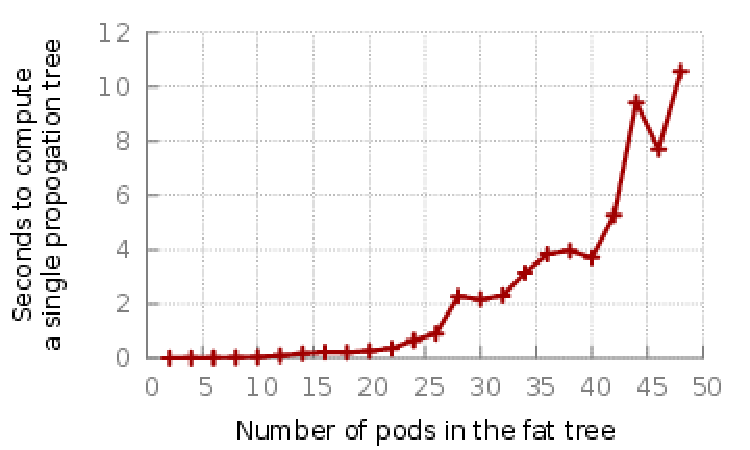
\includegraphics[width=3.25in]{../graphs/hsa_overhead_graph/graph.pdf}
    \caption[]{\label{fig:hsa_runtime} Serial runtime of correspondence
    checking on PORTLAND fat tree networks. Each datapoint consists of
    $x^3/4$ hosts and $5x^2/4$ switches (\eg{} 48 pods means 27,468 hosts
    attached to 2,880 switches)}
\end{figure}

\noindent{\bf Simulator Scalability.} Our design models the entire network
within a single process. We show in Figure~\ref{fig:scalability}
that this approach nonetheless scales to large networks. For this analysis we
generated fat tree topologies between 2 and 48 pods wide, where all switches in
the network connected to a single controller. The controller sent each switch
$FLOW_MOD$ and subsequent $BARRIER_REQUEST$ message, and waited for the
corresponding $BARRIER_REPLY$. We then measured the time to between the first
$FLOW_MOD$ sent and the last $BARRIER_REPLY$ received. As expected, the
runtime was roughly linear with the number of switches in the network. The
figure also shows that the processing time for large networks (5 seconds per
simulator round) was well within the bounds for interactive use.

\begin{figure}[t]
    %\hspace{-10pt}
    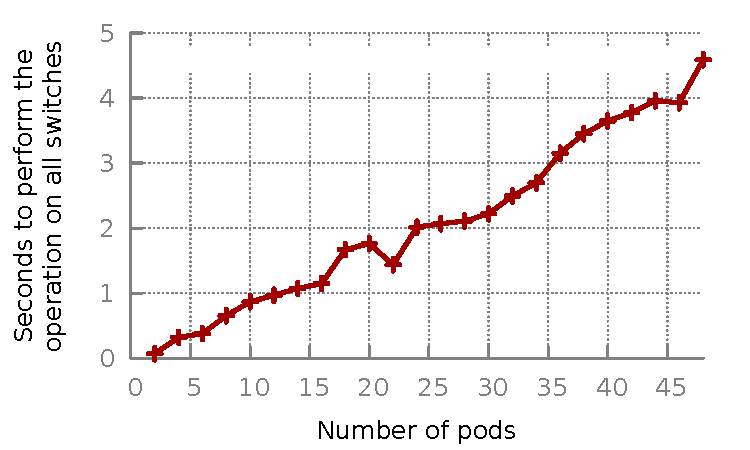
\includegraphics[width=3.25in]{../graphs/scalability_graph/scale.pdf}
    \caption[]{\label{fig:scalability} Time to send and process messages
    between controller and simulated switches. Each datapoint consists of
    $x^3/4$ hosts and $5x^2/4$ switches (\eg{} 48 pods means 27,468 hosts
    attached to 2,880 switches)}
\end{figure}

\subsection{Replay fidelity}

If our simulated model of the network is not sufficiently complex, it may not
be able to reproduce error conditions observed in production. Conversely,
resolving bugs observed in a simulated environment may not ensure
correct behavior of the production network. In future work, we hope to verify
the fidelity of \simulator{} by collaborating with industry partners to
reproduce bugs observed in practice. In addition, we
plan to gather error logs by deploying our own applications in Google's
datacenter networking research cluster~\cite{DNRC}.

Finally, note that our correspondence checking algorithm can not verify 
time-dependent policies such as ``No link should be congested more than 1\% of the
time'', or ``No server should receive more than 500MB/s of external traffic''.
In future work we will extend our correspondence checking algorithm to
account for this class of policies.
